\documentclass[11pt]{article}
\usepackage{amsmath,textcomp,amssymb,graphicx,comment,tikz}
\usepackage[margin=0.75in]{geometry}
\usetikzlibrary{arrows}
\newcommand{\tab}{\hspace*{2em}}

\def\Name{Alvin Wong, Wai Meng Lei, Chun Yin Yau}  % Your name

\title{CS189 --- Homework 6}
\author{\Name}
\markboth{CS189 Homework 6}{CS189 Homework 6}
\pagestyle{myheadings}

\begin{document}
\maketitle

\section*{1. Single-Layer Neural Network}

\textbf{ Derivation of gradient updates: }
\\\\\
Let $y_k = \sigma ( s_k  ) $, where $s_k  = \sum_j W_{jk} x_j + b_k $.
\\\\
1) Using the mean squared error: $J = \frac{1}{2} \sum_{k=1}^{n_{out}} (t_k - y_k)^2 $:
$$ \begin{aligned}
\frac{dJ}{d W_{jk} } &= \frac{d}{d W_{jk}} ( \frac{1}{2} \sum_{k=1}^{n_{out}} (t_k - y_k)^2 \\
&= (y_k - t_k) \frac{d}{d W_{jk}} \sigma(s_k) \\
&= (y_k - t_k) \sigma(s_k) (1 - \sigma(s_k)) \frac{d}{d W_jk} (W_{jk} x_j + b_k) \\
&= (y_k - t_k) \sigma(s_k) (1 - \sigma(s_k)) x_j 
\end{aligned} $$
$$ \begin{aligned}
\frac{dJ}{d b_j } &= \frac{d}{d b_j} ( \frac{1}{2} \sum_{k=1}^{n_{out}} (t_k - y_k)^2 \\
&= (y_k - t_k) \frac{d}{d b_j} \sigma(s_k) \\
&= (y_k - t_k) \sigma(s_k) (1 - \sigma(s_k)) \frac{d}{d b_j} (W_{jk} x_j + b_k) \\
&= (y_k - t_k) \sigma(s_k) (1 - \sigma(s_k)) 
\end{aligned} $$
In terms of matrices and vectors:
Let $\vec{y} = \sigma ( \vec{s} )$, and $\vec{s} = W \vec{x} + \vec{b} $:
$$ \boxed{\frac{dJ} {dW} = diag(\vec{y}) (1 - diag(\vec{y})) [ \vec{y} - \vec{t} ] \vec{x}^T} $$
$$ \boxed{\frac{dJ} {d\vec{b}} = diag(\vec{y}) (1 - diag(\vec{y})) [ \vec{y} - \vec{t} ]} $$
2) Using the cross-entropy error: $J = - \sum_{k=1}^{n_{out}} [t_k \ln y_k + (1 - t_k) \ln (1 - y_k)] $:
\\\\
The math works out the same, it's just the initial $y_k - t_k$ term becomes the derivative of the cross-entropy error term above:
$$ \frac{dJ}{d W_{jk} } = [ - \frac{t_k}{y_k} + \frac{1 - t_k}{1 - y_k} ] \sigma(s_k) (1 - \sigma(s_k)) x_j $$
$$ \frac{dJ}{d b_j } = [ - \frac{t_k}{y_k} + \frac{1 - t_k}{1 - y_k} ] \sigma(s_k) (1 - \sigma(s_k)) $$
In terms of matrices and vectors:
$$ \boxed{\frac{dJ} {dW} = diag(\vec{y}) (1 - diag(\vec{y})) [ - \frac{\vec{t}}{\vec{y}} + \frac{ 1 - \vec{t}}{1 - \vec{y}} ] \vec{x}^T} $$
$$ \boxed{\frac{dJ} {d\vec{b}} = diag(\vec{y}) (1 - diag(\vec{y})) [ - \frac{\vec{t}}{\vec{y}} + \frac{ 1 - \vec{t}}{1 - \vec{y}} ]} $$
\textbf{Figure 1: Plot of the training loss (blue) and test set accuracy (red), 500 epochs, MSE error}  \\
The test accuracy converged to 92.25\%. The total training loss converrged to about 4370. This took about a little over an hour to run.
\begin{figure}[ht!]
\centering
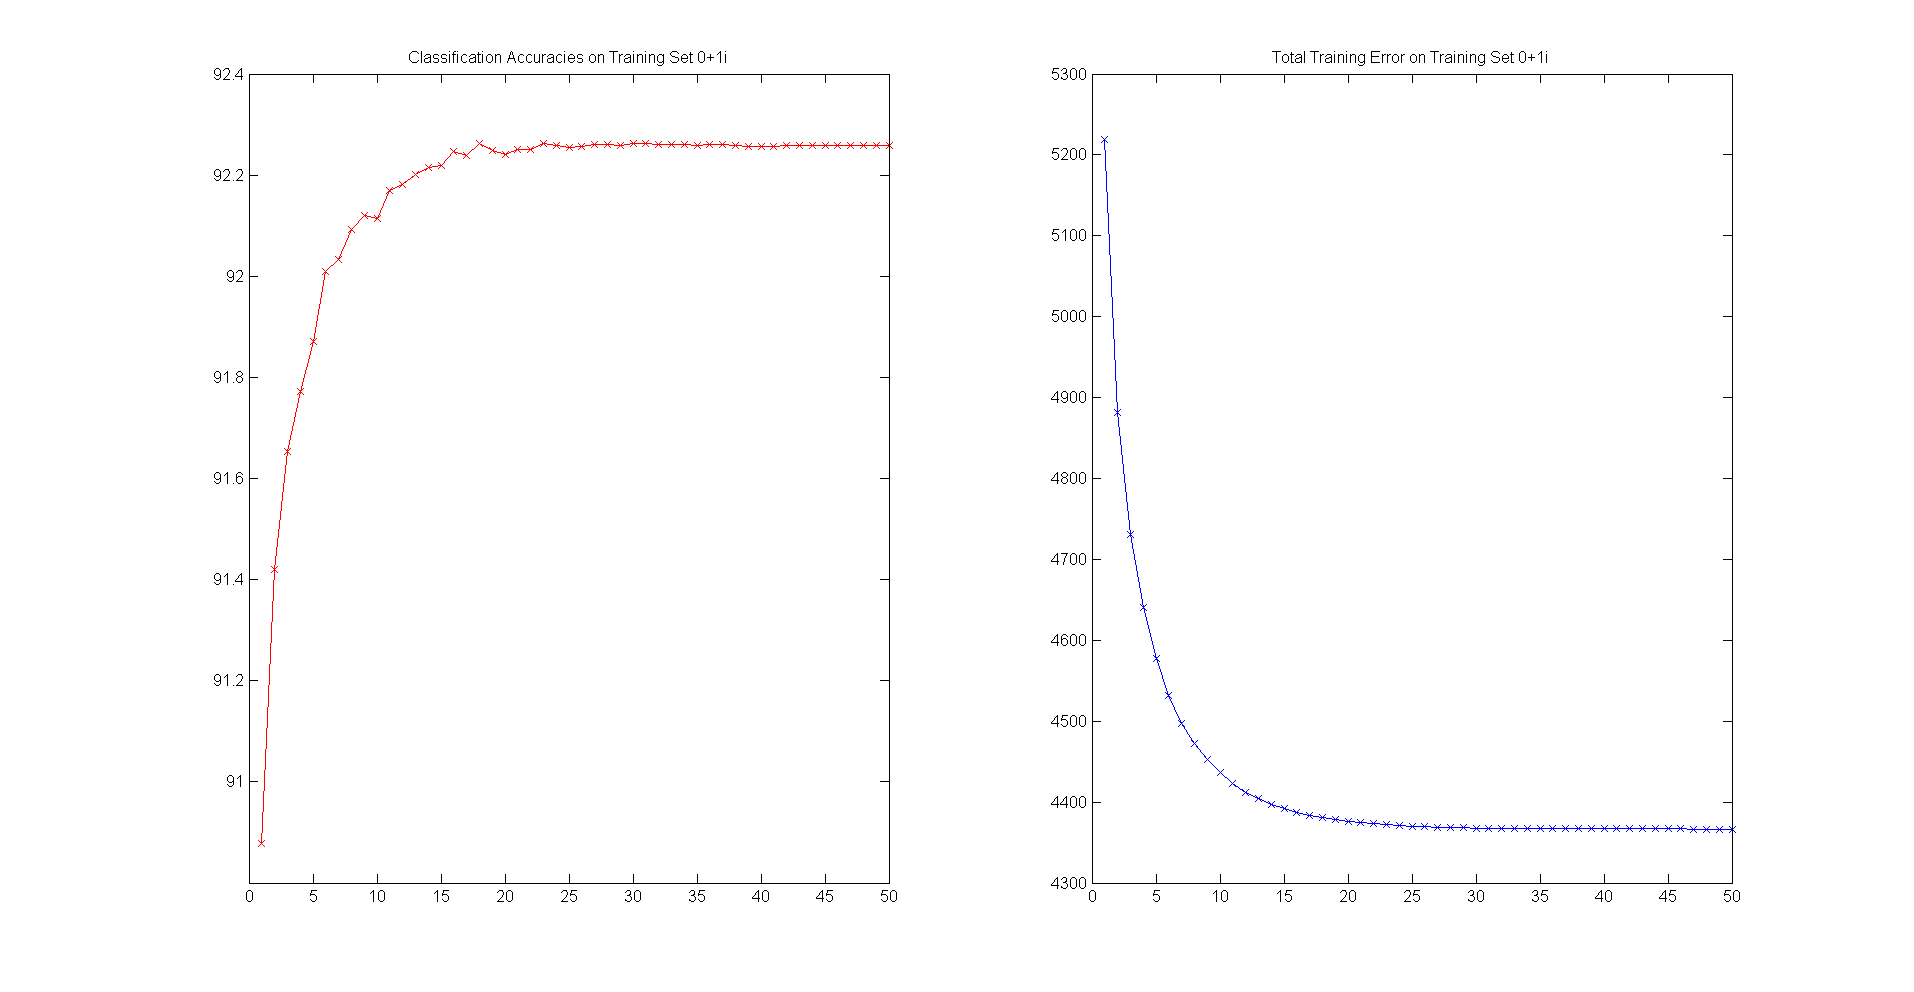
\includegraphics[width=150mm]{plots/finalp1mse.png}
\label{overflow}
\end{figure}
\\
\textbf{Figure 2: Plot of the training loss (blue) and test set accuracy (red), 500 epochs, CE error} \\
The test accuracy converged to 92.8\%. The total training loss converged to about 34300. This took about a little over an hour to run.
\begin{figure}[ht!]
\centering
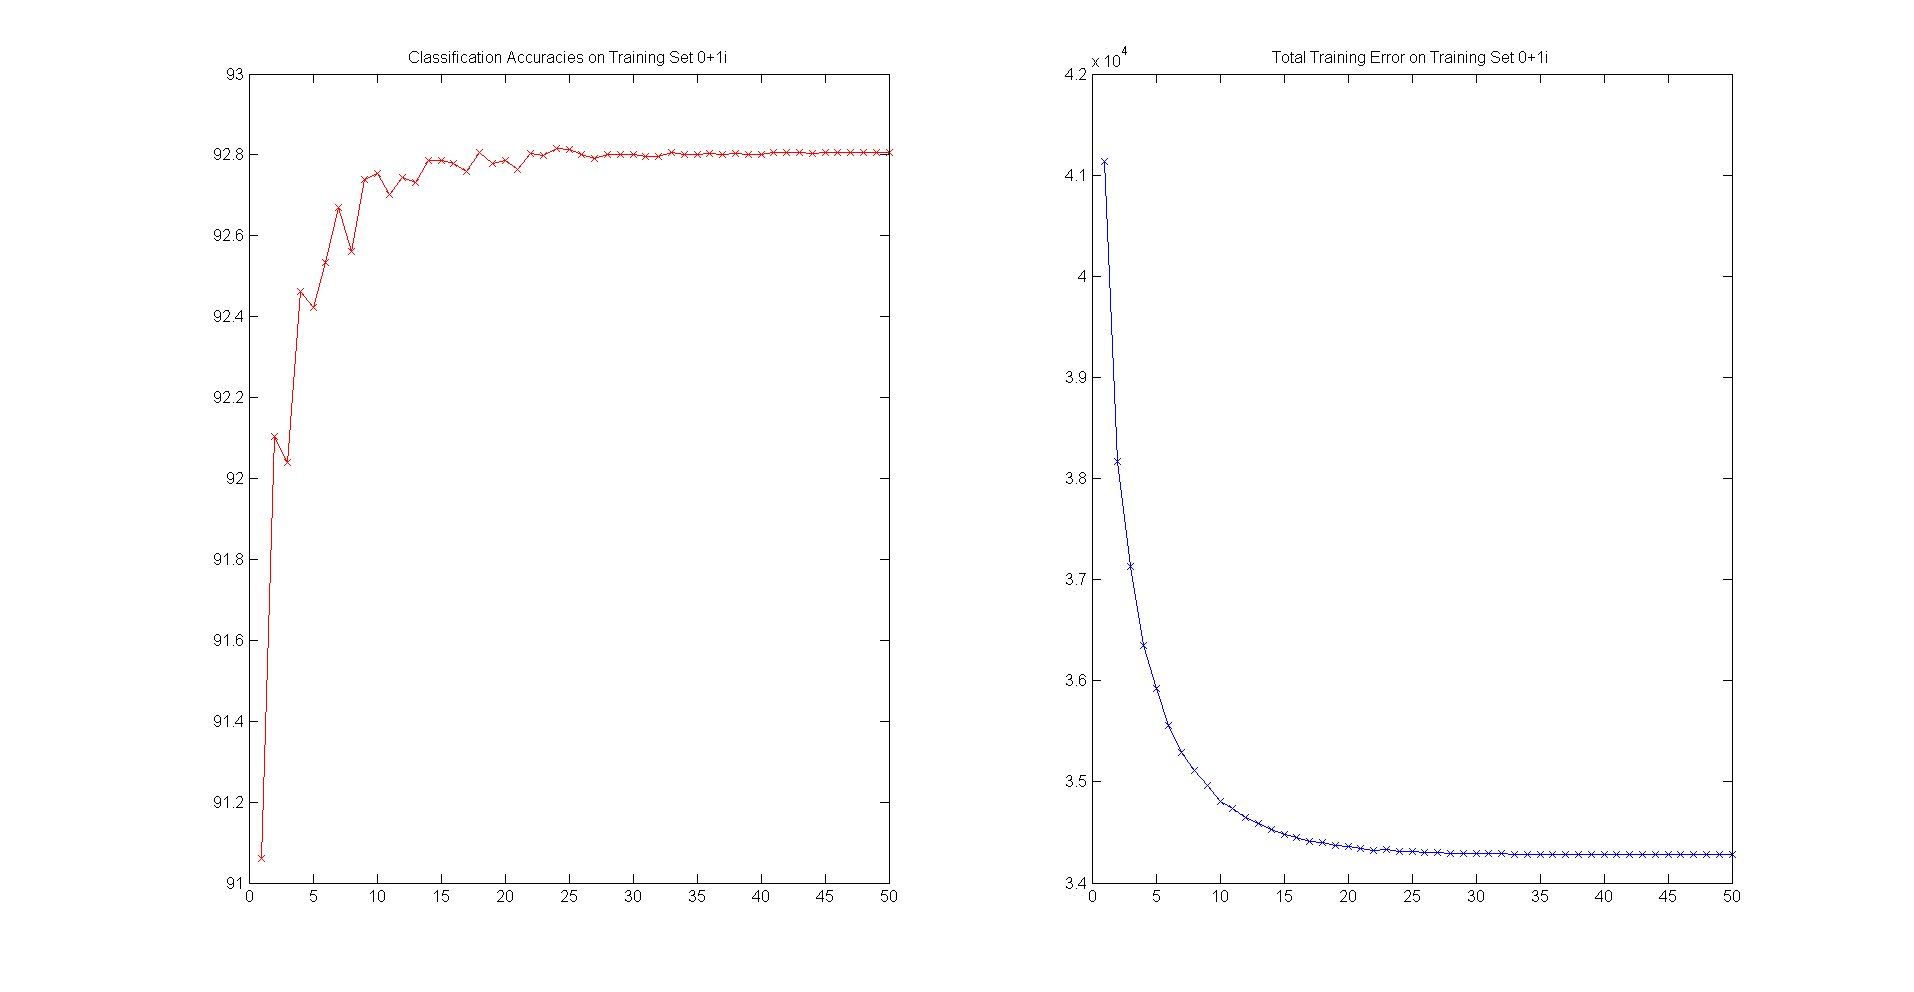
\includegraphics[width=150mm]{plots/finalp1ce.png}
\label{overflow}
\end{figure}
\\
Note: don't mind the titles -- they are wrong. Left graph is on test accuracy. Right graph is on training set loss.

\end{document}
